\documentclass[12pt]{beamer}

\usetheme{Air}
\usepackage[czech]{babel}
\usepackage[utf8x]{inputenc}

\title{Prostředí pro implementaci algoritmů Bayesovské filtrace}
\author[Matěj Laitl]{Matěj Laitl\\ vedoucí práce: Ing. Václav Šmídl, Ph.D.; ÚTIA}
\date{\today}

\begin{document}

\frame{\titlepage}

\section*{}
\begin{frame}
  \frametitle{Obsah}
  \tableofcontents[section=1,hidesubsections]
\end{frame}

\AtBeginSection[]
{
  \frame<handout:0>
  {
    \frametitle{Přehled}
    \tableofcontents[currentsection,hideallsubsections]
  }
}

\AtBeginSubsection[]
{
  \frame<handout:0>
  {
    \frametitle{Přehled}
    \tableofcontents[sectionstyle=show/hide,subsectionstyle=show/shaded/hide]
  }
}


%%%%%%%%%%%%%%%%%%%%%%%%%%%%%%%%%%%%%%%%%
%%%%%%%%%% Content starts here %%%%%%%%%%
%%%%%%%%%%%%%%%%%%%%%%%%%%%%%%%%%%%%%%%%%

\section*{Zadání}

\begin{frame}
	\frametitle{Zadání}

	\begin{block}{Úkoly práce}
		\begin{itemize}
			\item seznámit se s metodou rekurzivní Bayesovské identifikace (Bayesovské filtrace)
			\item softwarová analýza - vhodnost přístupů a programových prostředí
			\item implementace několika metod Bayesovské filtrace
			\item zveřejnění knihovny jako open-source projektu
		\end{itemize}
	\end{block}
\end{frame}

\section{Rekurzivní Bayesovská identifikace}

\begin{frame}
	\frametitle{Formulace problému 1/2}
	\framesubtitle{Dynamický systém}

	\begin{block}{model procesu}
		\(x_t = f(x_{t-1}, v_{t-1})\) \hspace{3cm} \(x_t\) .. stavový vektor

		\begin{itemize}
		\item \(v_t\) náhodný šum, iid
		\item → definuje pdf\footnote{hustota pravděpodobnosti} \(p(x_t|x_{t-1})\)
		\end{itemize}
	\end{block}

	\begin{block}{model pozorování}
		\(y_t = h(x_t, w_t)\) \hspace{3cm} \(y_t\) .. vektor pozorování

		\begin{itemize}
		\item \(w_t\) náhodný šum, iid
		\item → definuje pdf \(p(y_t|x_t)\)
		\end{itemize}
	\end{block}
\end{frame}

\begin{frame}
	\frametitle{Formulace problému 2/2}
	\framesubtitle{Cíle}

	{\large Úkol:
	\begin{itemize}
		\item odhadnout \(x_t\) z posloupnosti meření \(y_{1:t}\)
		\item precizněji: spočítat pdf \(p(x_t | y_{1:t})\)
	\end{itemize}
	}

	\begin{block}{Máme}
		\begin{itemize}
			\item \(p(x_t|x_{t-1})\) \hspace{1cm} speciálně \(p(x_0)\)
			\item \(p(y_t|x_t)\)
		\end{itemize}
	\end{block}

	\begin{example}
		\begin{itemize}
			\item robotika: lokalizace, sledování; avionika
			\item environmentální simulace: síření radioaktivního spadu
		\end{itemize}
	\end{example}
\end{frame}

% \begin{frame}
% 	\frametitle{Matematický aparát}
% 	\begin{block}{Řetězové pravidlo pro pdf}
% 		\[P(AB|C) = P(A|BC) P(B|C)\]
% 	\end{block}
% 
% 	\begin{block}{Bayesova věta}
% 		\[P(A|BC) = \frac{P(B|AC)P(A|C)}{P(B|C)}\]
% 	\end{block}
% 
% 	\begin{block}{Marginalizace pdf}
% 		\[p(x, y) = \int_{-\infty}^{\infty} p(x, y, z) \; \mathrm{d} z\]
% 	\end{block}
% \end{frame}

\begin{frame}
	\frametitle{Teoretické řešení}
	\framesubtitle{Rekurzivního algoritmus (zjednodušeno; Markovova vlastnost)}

	{\small Známe \(p(x_{t-1} | y_{1:t-1})\), odvoďme apriorní pdf \eqref{eq:PriorPdf}.}
	{\scriptsize (marg., řetěz. prav.)}
	\begin{align}
		p(x_t | y_{1:t-1}) &= \int_{-\infty}^{\infty} p(x_t, x_{t-1} | y_{1:t-1})
		\; \mathrm{d} x_{t-1} \notag \\
		%
		p(x_t | y_{1:t-1}) &= \int_{-\infty}^{\infty} p(x_t | x_{t-1}) p(x_{t-1} | y_{1:t-1})
		\; \mathrm{d} x_{t-1} \label{eq:PriorPdf}
	\end{align}

	{\small Přišlo pozorování \(y_t\), zakomponujme ho.}
	{\scriptsize (Bayesova věta)}
	\begin{align}
		p(x_t | y_{1:t}) &= \frac{p(y_t | x_t) p(x_t | y_{1:t-1})}{p(y_t | y_{1:t-1})}
		\label{eq:PosteriorPdf}
	\end{align}

	{\small Odvodili jsme aposteriorní pdf \eqref{eq:PosteriorPdf} pro \(x_t\).}
% 	Čitatel známý, jmenovatel je konstanta - buď netřeba nebo lze dopočítat marginalizací/z podmínky
% 	normality.
\end{frame}

\begin{frame}
	\frametitle{Problémy analytického řešení}
	\framesubtitle{Praktické metody Bayesovské filtrace}

	\begin{alertblock}{Problém!}
		Odvozené analytické řešení je velmi obtížné a nepraktické počítat pro více-dimenzionální
		systémy
	\end{alertblock}

	\begin{block}{Zjednodušení problému}
		\begin{itemize}
			\item Kalmanův filtr: Gaussovské šumy, lineární systém → zjednodušení
			na algebraické operace s kovariančními maticemi
		\end{itemize}
	\end{block}

	\begin{block}{Aproximace}
		\begin{itemize}
			\item Particle filtr: odhaduje aposteriorní pdf empirickou pdf,
			nedeterministický (Monte Carlo - samplování z pdf)
			\item Marginalizovaný particle filtr (Kalmanův + particle)
		\end{itemize}
	\end{block}

\end{frame}

\section{Výsledky softwarové analýzy}

\begin{frame}
	\frametitle{Východiska}

	{\large Cíl: vyvinout konkurenceschopnou knihovnu pro Bayesovské filtrování a jeho aplikace}

	\vspace{8mm}

	\begin{block}{Nejdůležitější požadavky}
		\begin{itemize}
			\item snadné a rychlé použití {\scriptsize (→ vysokoúrovňový jazyk)}
			\item rychlost {\scriptsize (v rozporu s předchozím)}
			\item rozšiřitelnost, přenositelnost, nezávislost na komerčních platformách
		\end{itemize}
 	\end{block}
\end{frame}

\begin{frame}
	\frametitle{Paradigmata, Programovací jazyky}

	\begin{block}{Vhodnost implementačních metodik}
		Objektově orientované programování nejlépe vystihuje matematickou strukturu teorie
	\end{block}

	\begin{block}{Implementační prostředí 1}
		\begin{itemize}
			\item C++
			\begin{itemize}
				\item + rozšířenost, rychlost, existující knihovny pro Bayes..
				\item - nízká produktivita, vysoké vstupní bariéry → nevhodné
			\end{itemize}
			\item Matlab
			\begin{itemize}
				\item + rozšířenost, vysoká produktivita
				\item - copy-on-write, nevhodné pro OOP, proprietární → nevhodný
			\end{itemize}
		\end{itemize}
	\end{block}
\end{frame}

\begin{frame}
	\frametitle{Programovací jazyky redux}

	\begin{block}{Implementační prostředí 2}
		\begin{itemize}
			\item Python
			\begin{itemize}
				\item + vysoká produktivita, existující mat. knihovny (NumPy), rozšířenost, komunita
				\item - vysoká režie (interpretovaný, dynamický jazyk) → sám o sobě nevhodný
			\end{itemize}
			\item Cython
			\begin{itemize}
				\item překládá Python kód do C
				\item \textbf{postupná} optimalizace stávajícího Python kódu
				\item naměřeno: 60x zrychlení pro numerickou integraci\footnote{dokazuje zejména
pomalost Pythonu}
				\item naměřeno: dodatečné 13x zrychlení při paralelizaci na 16-jádrovém CPU (OpenMP)
			\end{itemize}
		\end{itemize}
	\end{block}
\end{frame}

\begin{frame}
	\frametitle{Výkonnostní porovnání}
	\framesubtitle{C, Python, Cython, PyPy}

	Relativní rychlost numerické integrace
	\vspace{5mm}

	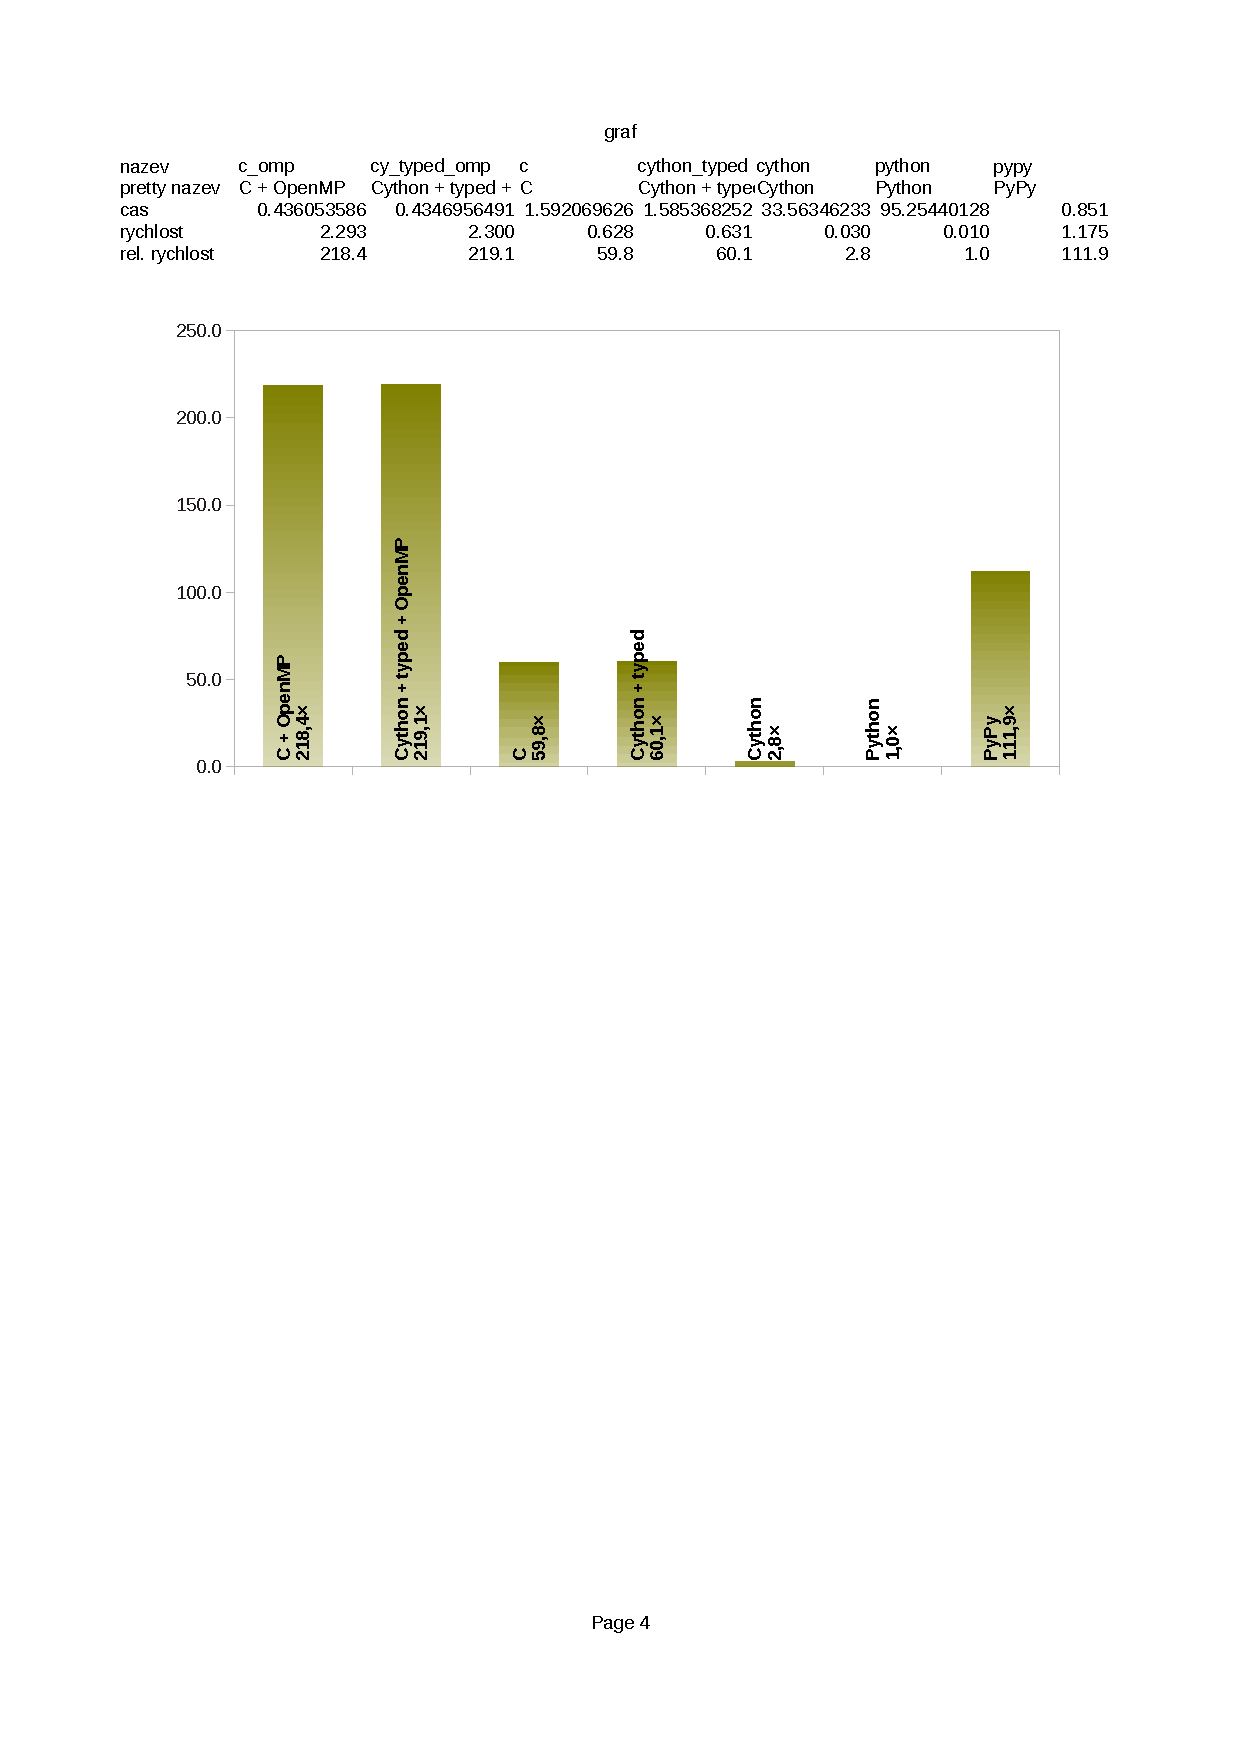
\includegraphics[width=\textwidth,keepaspectratio=true,clip=true,trim=30mm 166mm 30mm
54mm]{./edgy-results.pdf}
\end{frame}

\section{PyBayes}

\begin{frame}
	\frametitle{PyBayes}

	\begin{block}{PyBayes knihovna}
		\begin{itemize}
			\item open-source, otevřený vývoj na \url{http://github.com/strohel/PyBayes}
			\item možno interpretovat Pythonem / kompilovat Cythonem (optimalizace)
			\item Cython verze je 2 - 5x rychlejší
		\end{itemize}
	\end{block}

	\begin{block}{Implementováno v PyBayes}
		\begin{itemize}
			\item základní i podmíněné pdf, produkt pdf, řetězové pravidlo
			\item Kalmanův filtr, particle filtr, marginalizovaný PF
			\item kompletní dokumentace, unit-testy
		\end{itemize}
	\end{block}
\end{frame}

\begin{frame}
	\frametitle{Výkonnostní srovnání PyBayes}
	\framesubtitle{Čas na 3000 iterací Kalmanova filtru}

	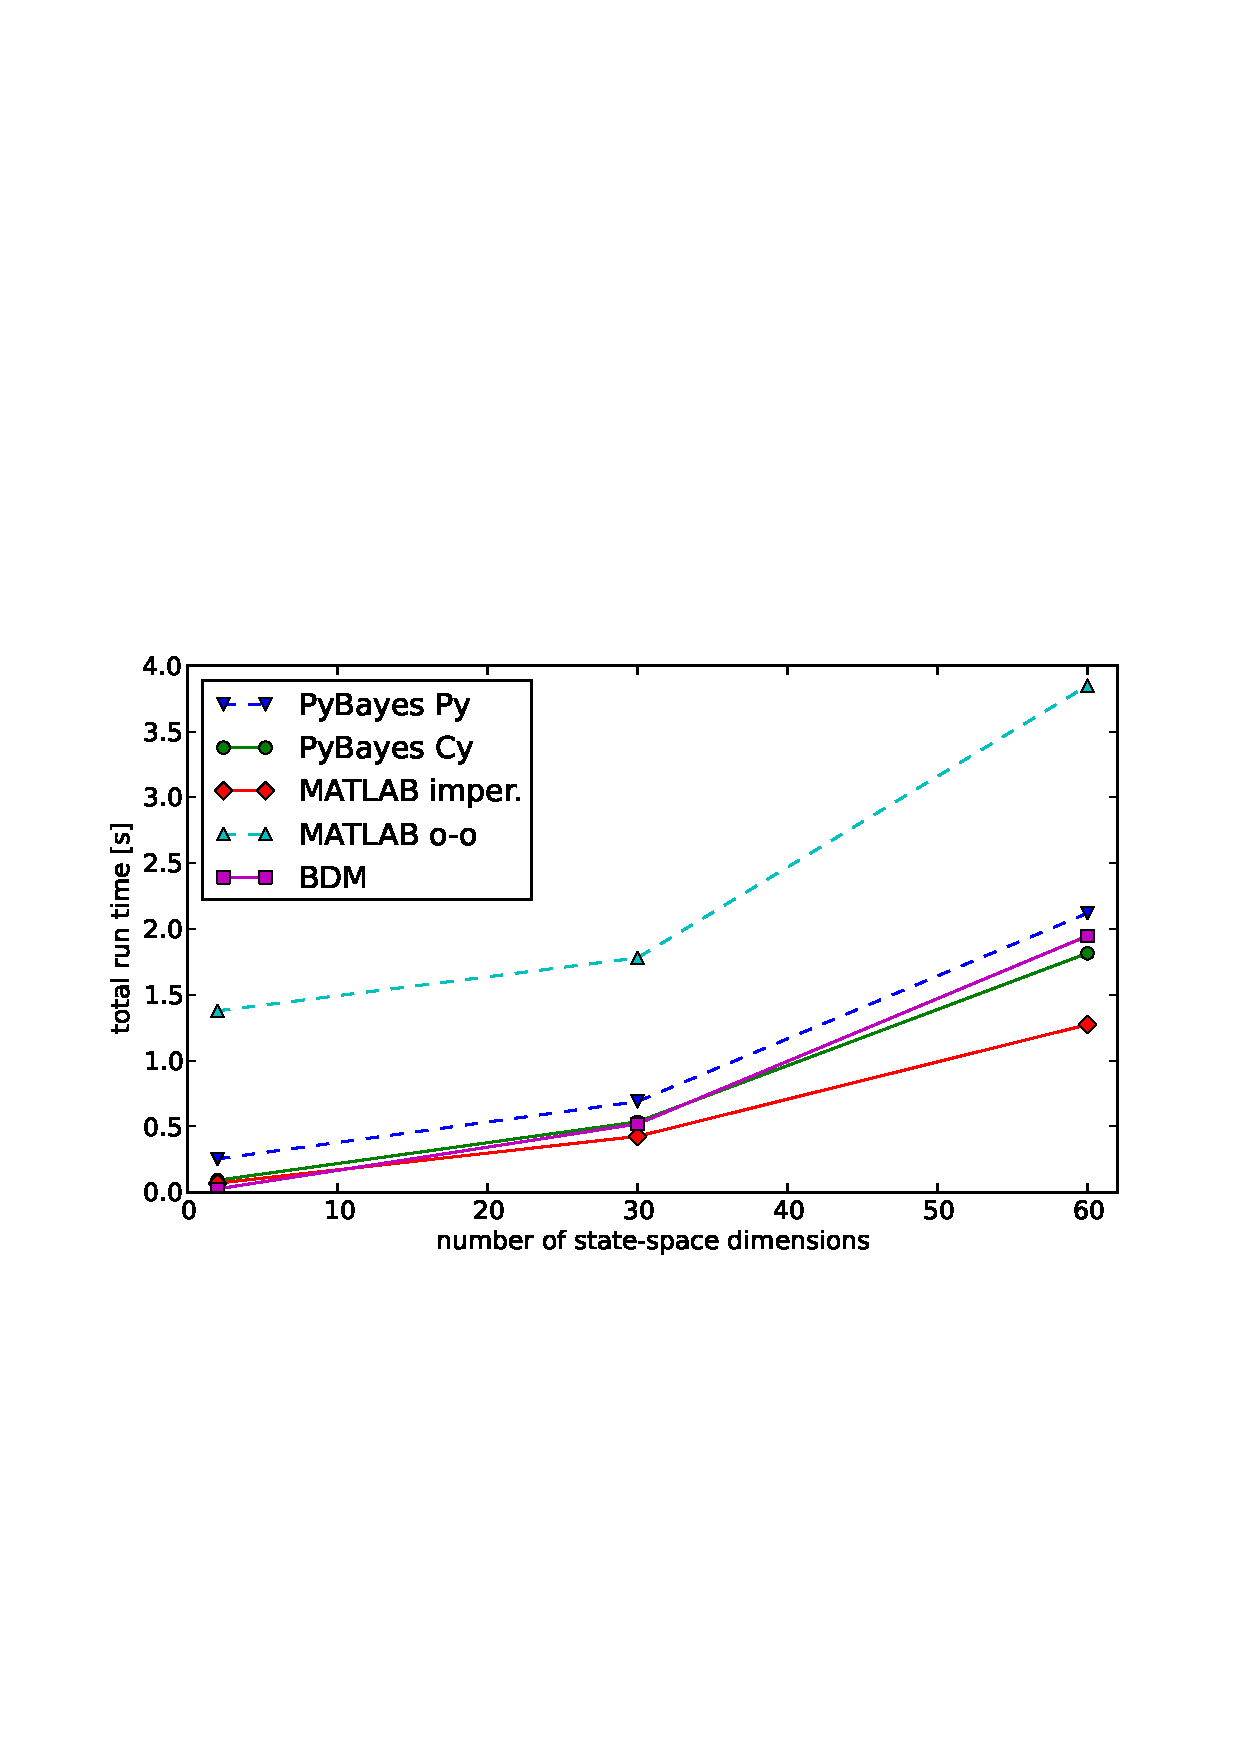
\includegraphics[width=\textwidth,keepaspectratio=true,clip=true,trim=19mm 85mm 20mm
111mm]{../KFPerf.pdf}
\end{frame}


\begin{frame}
	\begin{block}{Budoucnost}
		\begin{itemize}
			\item další filtrační metody: nelineární Kalmanovy filtry...
			\item další implementační prostředí: PyPy...
		\end{itemize}
	\end{block}

	\vspace{1cm}
	{\huge Děkuji za pozornost}

	\vspace{1cm}
	\begin{flushright}
		Matěj Laitl

		\structure{\footnotesize{matej@laitl.cz}}
	\end{flushright}
\end{frame}

\end{document}
